\documentclass[10pt,twocolumn,letterpaper]{article}

\usepackage{cvpr}
\usepackage{times}
\usepackage{epsfig}
\usepackage{graphicx}
\usepackage{amsmath}
\usepackage{amssymb}
\usepackage{url}
\usepackage{algorithm}% http://ctan.org/pkg/algorithms
\usepackage[noend]{algpseudocode}% http://ctan.org/pkg/algorithmicx
\usepackage{subcaption}

% Include other packages here, before hyperref.

% If you comment hyperref and then uncomment it, you should delete
% egpaper.aux before re-running latex.  (Or just hit 'q' on the first latex
% run, let it finish, and you should be clear).
\usepackage[breaklinks=true,bookmarks=false]{hyperref}

\cvprfinalcopy % *** Uncomment this line for the final submission

\def\cvprPaperID{****} % *** Enter the CVPR Paper ID here
\def\httilde{\mbox{\tt\raisebox{-.5ex}{\symbol{126}}}}

% Pages are numbered in submission mode, and unnumbered in camera-ready
%\ifcvprfinal\pagestyle{empty}\fi
\setcounter{page}{1}
\begin{document}

%%%%%%%%% TITLE
\title{Mathematical Expression Recognizer}

\author{ChanMin Kim \qquad HeeHoon Kim \qquad Sanghyeok Park\\
Department of Computer Science and Engineering\\
Seoul National University\\
{\tt\small kcm1700@snu.ac.kr, csehydrogen@gmail.com, pps987@snu.ac.kr}
% For a paper whose authors are all at the same institution,
% omit the following lines up until the closing ``}''.
% Additional authors and addresses can be added with ``\and'',
% just like the second author.
% To save space, use either the email address or home page, not both
}

\maketitle
%\thispagestyle{empty}

%%%%%%%%% ABSTRACT
\begin{abstract}
	TODO:
\end{abstract}

%%%%%%%%% BODY TEXT
\section{Introduction}

We implemented a simple mathematical expression recognizer which takes pictures of
math expressions and generates TeX form of expressions. Our program has some restrictions.
It can only recognize expressions that has only digits, arithmetic operators($+, -, *, /, \div$),
parentheses, $\pi$, $e$. Expressions also should be in one line, and not have
superscripts or subscripts. Background should be bright, and the expression should be dark.

We devided this problem into three parts, normalization, segmentation, and recognition.
In normalization part, we binarized our gray scale natural image, and rotated it to
fit in straight rectangle box. In binarization, we applied local thresholding method.
Then we use ternary search method to find best angle we have to rotate.

In segmentation part, basically we splited binarized symbols into connected components
using Flood-Fill. However, we had to merge components into same symbol. For example,
$=$ symbol is one symbol but it has two components. Because our expressions is in only
one line, we measured only X-coordinates and overlap ratio of components. If one of the
two components overlap ratio is larger than the threshold, we merged those components
into same symbol. We chose the threshold $50\%$.

In recognition part, we determined which symbol each merged component actually is. The probability for each component to be a specific symbol was calculated from neural network. Our neural network model is modified LeNet\cite{LeNet}. The network was trained and tested with Caffe, using MNIST\cite{MNIST} and CROHME\cite{CROHME} data sets. In order to prevent nonsense predictions (consecutive operators, unmatched parentheses, etc.), we used dynamic programming approach.

% TODO
% result & this research's contribution (accomplishment) to this field

\section{Background}

There are a number of prior studies in the field of recognition of mathematical expressions.

Michael Nielsen\cite{MichaelNielsen} wrote an introductory book on neural networks.
The book describes the basics of neural network.

MNIST\cite{MNIST} data sets are famous for handwritten digits.

One of the most popular mathematical expression recognition competition is CROHME,
which stands for
`Competition on Recognition of Online Handwritten Mathematical Expressions'\cite{CROHME}.
They provide rich train data set and test data set of handwritten mathematical expressions
in InkML. InkML is a file format for representing trace of handwriting.


There was a student project by Vitali Sepetnitsky and Yakir Dahan\cite{OCRMATH}, which recognizes book printed mathematical formulas.
There was also a related course project by Alistair Dobke and Mark Mann\cite{OCRMATH2}. The project recognizes handwritten mathematical expressions just as our project.



\section{Approach}

% TODO:
% 우리들의 문제 해결은 어떻게 했는지 쓰기. 여기를 심혈을 기울여 쓰는 게 맞을듯
%
% 생각하고 있는 구조.
%
% - 알고리즘 (중요)
%  - neural net training
%    - training/test 데이터 가공
%    - 사용한 파라미터와 구조 설명(conv1,conv2,conv3,ReLU,inner product, dropout, output layer(softmax) 언급 다 필요. conv는 kernel size 및 개수 표현)
%  - normalization
%    - binarization: local threshold method 알고리즘 구체적으로 설명. 이미지 또는 pseudo code 필요
%    - rotation: 수식으로 설명. ternary search는 언급하면 될듯
%  - segmentation
%    - flood fill
%    - merging intervals 알고리즘 설명 및 PPT 이미지 활용
%    - dot recognition: 최대 높이/ 최저 높이 추정하고 그것을 기준으로 점 여부 판별하고 위치에 따라 .과 \cdot 분리
%  - dynamic programming
%    - 불가능한 수식 거르는 규칙
%      - 괄호
%      - opening parenthesis '(' 직후 binary 연산자(unary는 허용) 확률 0
%      - closing parenthesis ')' 직후 binary 연산자(unary는 허용) 확률 0
%      - 등 다양한 규칙 썼는데, 이걸 서술할 것.
%    - softmax 결과를 이용한 확률 곱 최대화.
%    - DP state 정의 및 의미
%    - 기대되는 효과: 실제 digit 단위 실험 결과를 보면 confusion matrix에서 /,(,),1 등이 자주 헷갈리고 3,{가 헷갈리고, 9,}가 헷갈리는데 이러한 경우 어느 게 맞는지 효과적으로 추론.
% - 프로그래밍 언어: python
% - 사용한 내용: caffe(뉴럴넷), Pillow(이미지 처리용), numpy(각종 계산용), scipy(마찬가지), django(웹데모개발용)
%
%
%
%

% TODO: 여기다가 Approach section의 구조 설명을 추가한다.

\subsection{Algorithm}

Our algorithm consists of several steps. We first binarize the image and rotate the image.
Then we segment the image into characters.
The final step is to apply dynamic programming to guess each symbols.

\subsubsection{Single Digit Recognition by Convolutional Neural Network}

\subsubsection{Binarization}

\begin{algorithm}
\caption{Binarization} \label{binarization}
\begin{algorithmic}[1]
\Function{binarize}{}
\State \texttt{image} $\gets$ grayscale(\texttt{image})
\State \texttt{ns} $\gets$ \textbf{max} (2, \texttt{width} / 350, \texttt{height} / 350)
\State \texttt{nearsum} $\gets$ \texttt{image} $\ast$ (\texttt{ns} $\times$ \texttt{ns} mean filter) \\
\Comment{$\ast$: convolution operator}
\State \texttt{fs} $\gets$ \textbf{max} (10, \texttt{width} / 30, \texttt{height} / 30)
\State \texttt{farsum} $\gets$ \texttt{image} $\ast$ (\texttt{fs} $\times$ \texttt{fs} mean filter)
\State \texttt{threshold} $\gets \frac{1}{6}$ min (\texttt{nearsum} - \texttt{farsum})
\State \Return \texttt{nearsum} $<$ \texttt{farsum} + \texttt{threshold}
\EndFunction
\end{algorithmic}
\end{algorithm}

The binarization algorithm consists of several steps as shown in \textbf{Algorithm \ref{binarization}}.
The algorithm caculates nearby pixel average and wider area average for each pixel.
Then the function calculates the differences and check the difference against the \texttt{threshold}.
The result is \texttt{height} $\times$ \texttt{width} binarized image.

\begin{figure}[t]
\begin{center}
   \subcaptionbox{global thresholding}{
        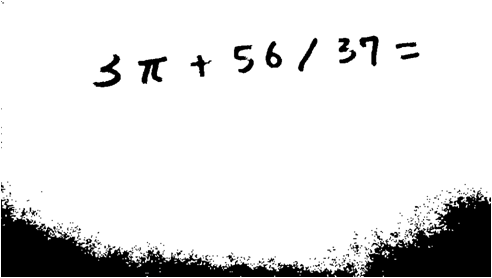
\includegraphics[width=0.47\linewidth]{img/global.png}
   }
   \subcaptionbox{local thresholding}{
       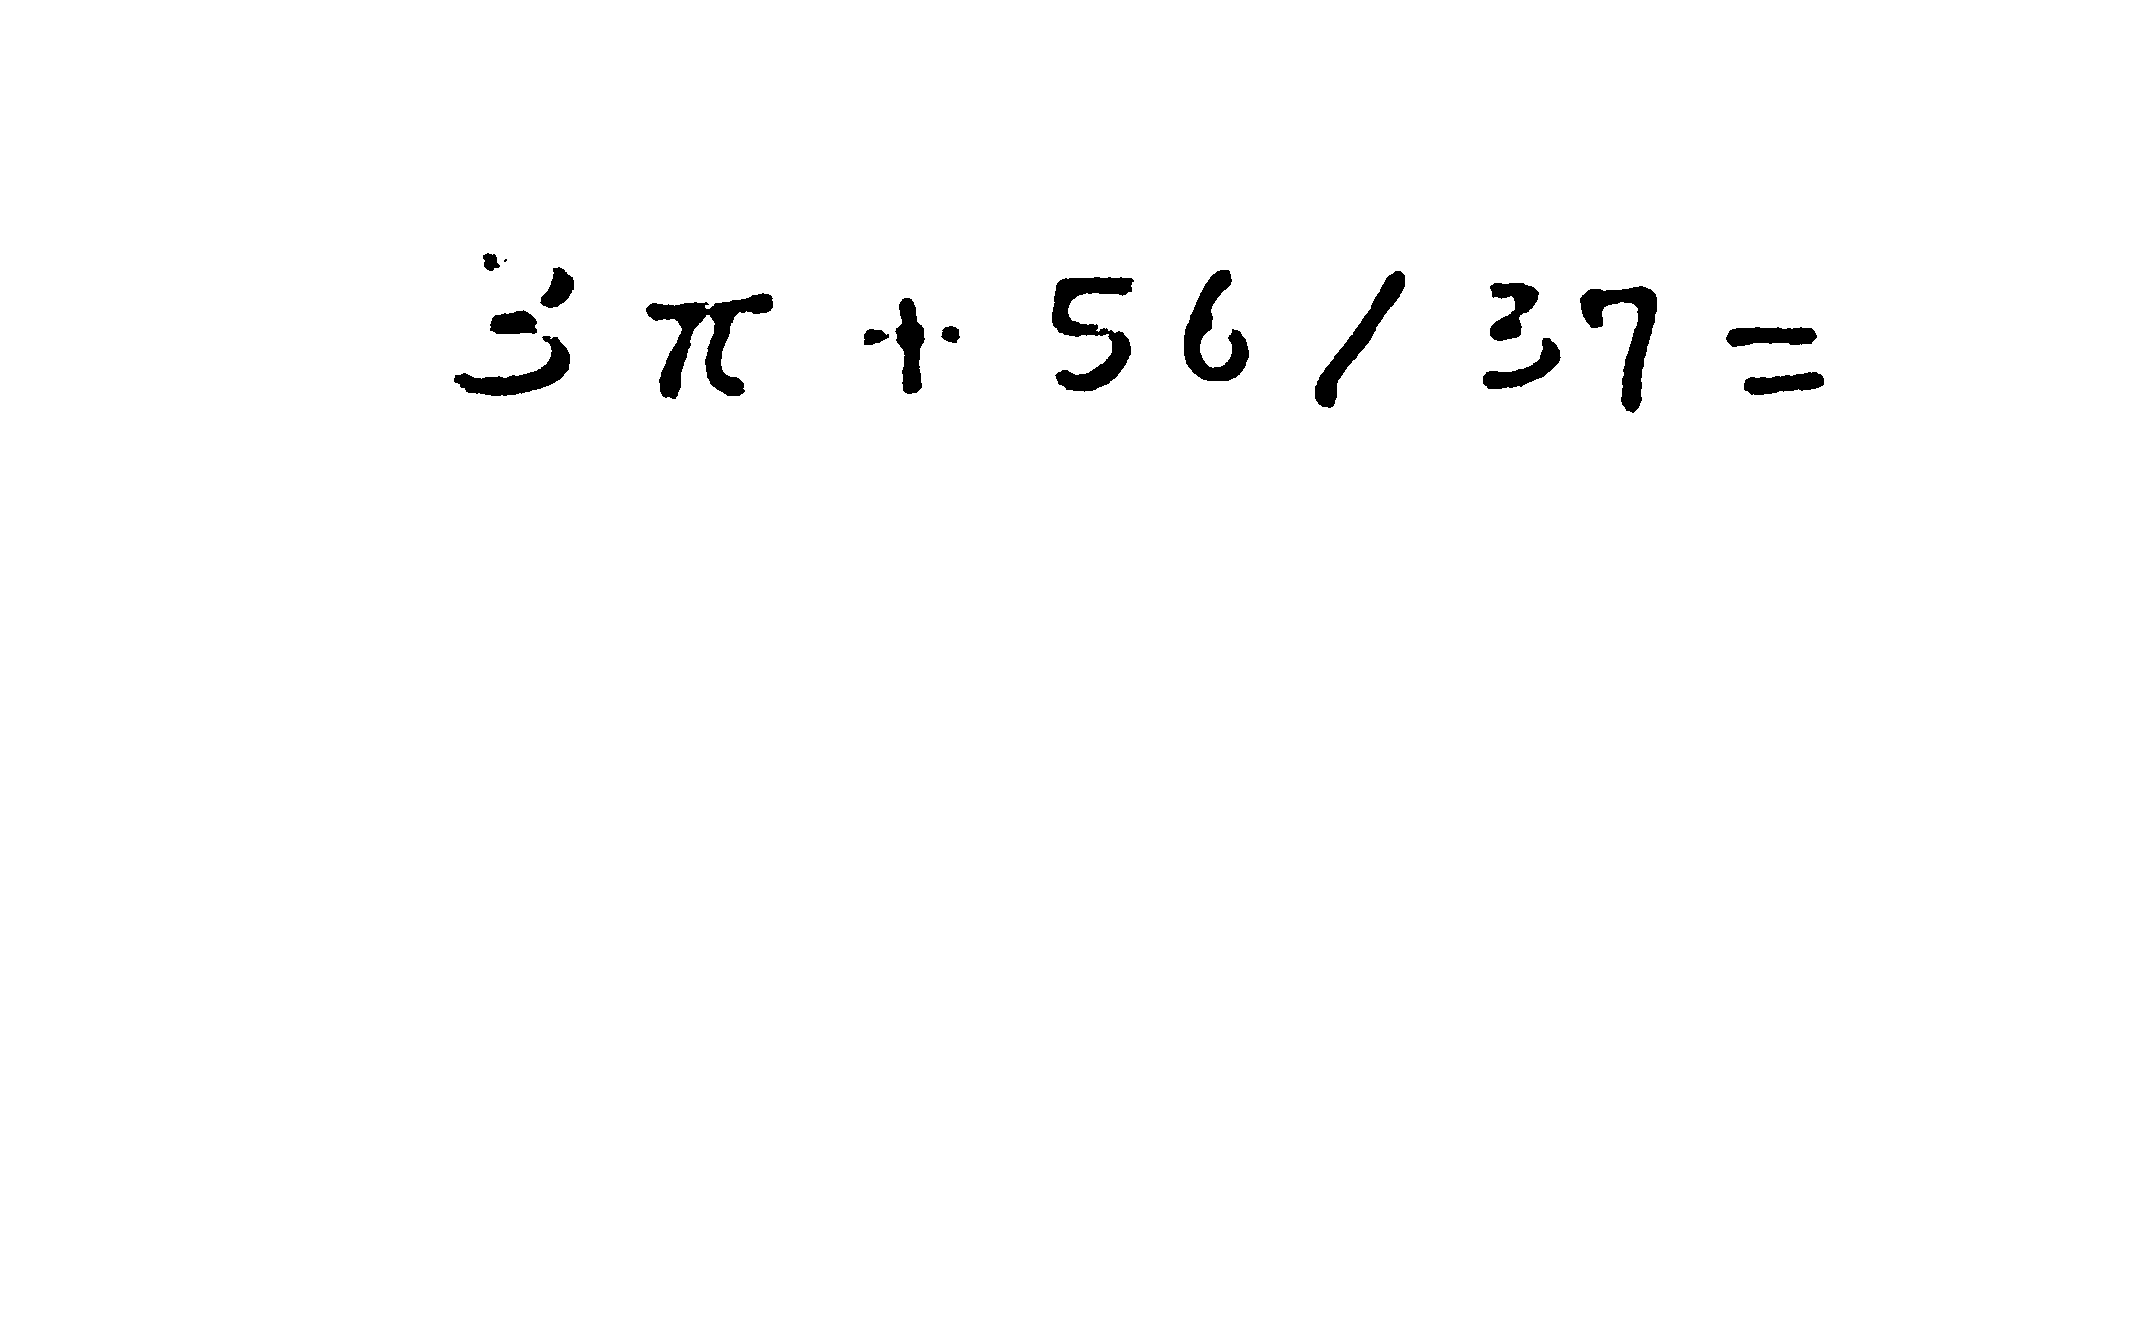
\includegraphics[width=0.47\linewidth]{img/local.png}
   }
\end{center}
   \caption{It is nearly impossible to separate the text by usual thresholding methods. }
\label{fig:thresholding}
\end{figure}

Our binarization method uses only neighborhood information.
We were forced to apply local thresholding method instead of global thresholding method.
Some parts of the background were sometimes darker than the text.
See Figure \ref{fig:thresholding} for example.



\subsubsection{Rotation}

\subsubsection{Flood Fill}

\subsubsection{Region Merge}

\subsubsection{Dynamic Programming}

\subsection{Environments}

We used Python 2.7 as our main programming language.
We used caffe and its python library for neural network.
We used Pillow for basic image manipulation and numpy \& scipy for faster calculation.
We used Django web framework for the web demo.

\section{Experiments}
%
% 여기다 적을 거
%
% 1. symbol recognition 결과
% 방법:
%   Dataset: CROHME 것을 사용한다. inkml 파일에서 우리가 대상으로 하는 symbol만 추린다. 굵기 별로 생성한다. 학습에 CROHME의 training set 사용. 평가에 CROHME의 test set 사용함.
%   softmax로 나온 결과 layer에서 argmax가 실제랑 같은지 비교
% 결과:
%   Neural Network 학습 결과 filter visualize
%   Neural Network 학습 결과 실제 샘플 convolution 결과 테이블.
%   confusion matrix. 그리고 confusion matrix의 자주 틀리는 부분들 이유 간략히 서술.
%   전체 정확도 및 신뢰 구간 구하기.
%
% 2. 실제 이미지 입력 (모두 web demo에서 참고하기) 이건 qualitative밖에 얘기 못할듯. 주목할만한 오류들 적기.
%   방법: 수식을 제시하고 해당 수식을 몇 명에게 handwriting을 받아서 수행
%
%


The web demo is available at \url{http://chanmin.kim/image-expr/}.

\section{Conclusion}

{\small
\bibliographystyle{ieee}
\bibliography{egbib}
}

\section{Appendices}

\begin{table}[h]
\centering
\label{symbol-list}
\begin{tabular}{|l|l|l|l|l|l|l|}
\hline
$($ & $)$ & $+$ & $-$ & $/$ & 0 & 1 \\ \hline
2 & 3 & 4 & 5 & 6 & 7 & 8 \\ \hline
9 & $=$ & $[$ & $\div$ & $\pi$ & $\times$ & $\{$ \\ \hline
$\}$ & $]$ & e & $\cdot$ & $.$ & & \\
\hline
\end{tabular}
\caption{List of recognizable symbols}
\end{table}



%-------------------------------------------------------------------------
\subsection{Language}

All manuscripts must be in English.

\subsection{Dual submission}

Please refer to the author guidelines on the CVPR 2015 web page for a
discussion of the policy on dual submissions.

\subsection{Paper length}
For CVPR 2015, the rules about paper length have changed, so please
read this section carefully. Papers, excluding the references section,
must be no longer than eight pages in length. The references section
will not be included in the page count, and there is no limit on the
length of the references section. For example, a paper of eight pages
with two pages of references would have a total length of 10 pages.
{\bf Unlike previous years, there will be no extra page charges for
  CVPR 2015.}

Overlength papers will simply not be reviewed.  This includes papers
where the margins and formatting are deemed to have been significantly
altered from those laid down by this style guide.  Note that this
\LaTeX\ guide already sets figure captions and references in a smaller font.
The reason such papers will not be reviewed is that there is no provision for
supervised revisions of manuscripts.  The reviewing process cannot determine
the suitability of the paper for presentation in eight pages if it is
reviewed in eleven.  

%-------------------------------------------------------------------------
\subsection{The ruler}
The \LaTeX\ style defines a printed ruler which should be present in the
version submitted for review.  The ruler is provided in order that
reviewers may comment on particular lines in the paper without
circumlocution.  If you are preparing a document using a non-\LaTeX\
document preparation system, please arrange for an equivalent ruler to
appear on the final output pages.  The presence or absence of the ruler
should not change the appearance of any other content on the page.  The
camera ready copy should not contain a ruler. (\LaTeX\ users may uncomment
the \verb'\cvprfinalcopy' command in the document preamble.)  Reviewers:
note that the ruler measurements do not align well with lines in the paper
--- this turns out to be very difficult to do well when the paper contains
many figures and equations, and, when done, looks ugly.  Just use fractional
references (e.g.\ this line is $095.5$), although in most cases one would
expect that the approximate location will be adequate.

\subsection{Mathematics}

Please number all of your sections and displayed equations.  It is
important for readers to be able to refer to any particular equation.  Just
because you didn't refer to it in the text doesn't mean some future reader
might not need to refer to it.  It is cumbersome to have to use
circumlocutions like ``the equation second from the top of page 3 column
1''.  (Note that the ruler will not be present in the final copy, so is not
an alternative to equation numbers).  All authors will benefit from reading
Mermin's description of how to write mathematics:
\url{http://www.pamitc.org/documents/mermin.pdf}.


\subsection{Blind review}

Many authors misunderstand the concept of anonymizing for blind
review.  Blind review does not mean that one must remove
citations to one's own work---in fact it is often impossible to
review a paper unless the previous citations are known and
available.

Blind review means that you do not use the words ``my'' or ``our''
when citing previous work.  That is all.  (But see below for
techreports.)

Saying ``this builds on the work of Lucy Smith [1]'' does not say
that you are Lucy Smith; it says that you are building on her
work.  If you are Smith and Jones, do not say ``as we show in
[7]'', say ``as Smith and Jones show in [7]'' and at the end of the
paper, include reference 7 as you would any other cited work.

An example of a bad paper just asking to be rejected:
\begin{quote}
\begin{center}
    An analysis of the frobnicatable foo filter.
\end{center}

   In this paper we present a performance analysis of our
   previous paper [1], and show it to be inferior to all
   previously known methods.  Why the previous paper was
   accepted without this analysis is beyond me.

   [1] Removed for blind review
\end{quote}


An example of an acceptable paper:

\begin{quote}
\begin{center}
     An analysis of the frobnicatable foo filter.
\end{center}

   In this paper we present a performance analysis of the
   paper of Smith \etal [1], and show it to be inferior to
   all previously known methods.  Why the previous paper
   was accepted without this analysis is beyond me.

   [1] Smith, L and Jones, C. ``The frobnicatable foo
   filter, a fundamental contribution to human knowledge''.
   Nature 381(12), 1-213.
\end{quote}

If you are making a submission to another conference at the same time,
which covers similar or overlapping material, you may need to refer to that
submission in order to explain the differences, just as you would if you
had previously published related work.  In such cases, include the
anonymized parallel submission~\cite{Authors14} as additional material and
cite it as
\begin{quote}
[1] Authors. ``The frobnicatable foo filter'', F\&G 2014 Submission ID 324,
Supplied as additional material {\tt fg324.pdf}.
\end{quote}

Finally, you may feel you need to tell the reader that more details can be
found elsewhere, and refer them to a technical report.  For conference
submissions, the paper must stand on its own, and not {\em require} the
reviewer to go to a techreport for further details.  Thus, you may say in
the body of the paper ``further details may be found
in~\cite{Authors14b}''.  Then submit the techreport as additional material.
Again, you may not assume the reviewers will read this material. 

Sometimes your paper is about a problem which you tested using a tool which
is widely known to be restricted to a single institution.  For example,
let's say it's 1969, you have solved a key problem on the Apollo lander,
and you believe that the CVPR70 audience would like to hear about your
solution.  The work is a development of your celebrated 1968 paper entitled
``Zero-g frobnication: How being the only people in the world with access to
the Apollo lander source code makes us a wow at parties'', by Zeus \etal.

You can handle this paper like any other.  Don't write ``We show how to
improve our previous work [Anonymous, 1968].  This time we tested the
algorithm on a lunar lander [name of lander removed for blind review]''.
That would be silly, and would immediately identify the authors. Instead
write the following:
\begin{quotation}
\noindent
   We describe a system for zero-g frobnication.  This
   system is new because it handles the following cases:
   A, B.  Previous systems [Zeus et al. 1968] didn't
   handle case B properly.  Ours handles it by including
   a foo term in the bar integral.

   ...

   The proposed system was integrated with the Apollo
   lunar lander, and went all the way to the moon, don't
   you know.  It displayed the following behaviours
   which show how well we solved cases A and B: ...
\end{quotation}
As you can see, the above text follows standard scientific convention,
reads better than the first version, and does not explicitly name you as
the authors.  A reviewer might think it likely that the new paper was
written by Zeus \etal, but cannot make any decision based on that guess.
He or she would have to be sure that no other authors could have been
contracted to solve problem B.

FAQ: Are acknowledgements OK?  No.  Leave them for the final copy.


\begin{figure}[t]
\begin{center}
\fbox{\rule{0pt}{2in} \rule{0.9\linewidth}{0pt}}
   %\includegraphics[width=0.8\linewidth]{egfigure.eps}
\end{center}
   \caption{Example of caption.  It is set in Roman so that mathematics
   (always set in Roman: $B \sin A = A \sin B$) may be included without an
   ugly clash.}
\label{fig:long}
\label{fig:onecol}
\end{figure}

\subsection{Miscellaneous}

\noindent
Compare the following:\\
\begin{tabular}{ll}
 \verb'$conf_a$' &  $conf_a$ \\
 \verb'$\mathit{conf}_a$' & $\mathit{conf}_a$
\end{tabular}\\
See The \TeX book, p165.

The space after \eg, meaning ``for example'', should not be a
sentence-ending space. So \eg is correct, {\em e.g.} is not.  The provided
\verb'\eg' macro takes care of this.

When citing a multi-author paper, you may save space by using ``et alia'',
shortened to ``\etal'' (not ``{\em et.\ al.}'' as ``{\em et}'' is a complete word.)
However, use it only when there are three or more authors.  Thus, the
following is correct: ``
   Frobnication has been trendy lately.
   It was introduced by Alpher~\cite{Alpher02}, and subsequently developed by
   Alpher and Fotheringham-Smythe~\cite{Alpher03}, and Alpher \etal~\cite{Alpher04}.''

This is incorrect: ``... subsequently developed by Alpher \etal~\cite{Alpher03} ...''
because reference~\cite{Alpher03} has just two authors.  If you use the
\verb'\etal' macro provided, then you need not worry about double periods
when used at the end of a sentence as in Alpher \etal.

For this citation style, keep multiple citations in numerical (not
chronological) order, so prefer \cite{Alpher03,Alpher02,Authors14} to
\cite{Alpher02,Alpher03,Authors14}.


\begin{figure*}
\begin{center}
\fbox{\rule{0pt}{2in} \rule{.9\linewidth}{0pt}}
\end{center}
   \caption{Example of a short caption, which should be centered.}
\label{fig:short}
\end{figure*}

%------------------------------------------------------------------------
\section{Formatting your paper}

All text must be in a two-column format. The total allowable width of the
text area is $6\frac78$ inches (17.5 cm) wide by $8\frac78$ inches (22.54
cm) high. Columns are to be $3\frac14$ inches (8.25 cm) wide, with a
$\frac{5}{16}$ inch (0.8 cm) space between them. The main title (on the
first page) should begin 1.0 inch (2.54 cm) from the top edge of the
page. The second and following pages should begin 1.0 inch (2.54 cm) from
the top edge. On all pages, the bottom margin should be 1-1/8 inches (2.86
cm) from the bottom edge of the page for $8.5 \times 11$-inch paper; for A4
paper, approximately 1-5/8 inches (4.13 cm) from the bottom edge of the
page.

%-------------------------------------------------------------------------
\subsection{Margins and page numbering}

All printed material, including text, illustrations, and charts, must be kept
within a print area 6-7/8 inches (17.5 cm) wide by 8-7/8 inches (22.54 cm)
high.
Page numbers should be in footer with page numbers, centered and .75
inches from the bottom of the page and make it start at the correct page
number rather than the 4321 in the example.  To do this fine the line (around
line 23)
\begin{verbatim}
%\ifcvprfinal\pagestyle{empty}\fi
\setcounter{page}{4321}
\end{verbatim}
where the number 4321 is your assigned starting page.

Make sure the first page is numbered by commenting out the first page being
empty on line 46
\begin{verbatim}
%\thispagestyle{empty}
\end{verbatim}


%-------------------------------------------------------------------------
\subsection{Type-style and fonts}

Wherever Times is specified, Times Roman may also be used. If neither is
available on your word processor, please use the font closest in
appearance to Times to which you have access.

MAIN TITLE. Center the title 1-3/8 inches (3.49 cm) from the top edge of
the first page. The title should be in Times 14-point, boldface type.
Capitalize the first letter of nouns, pronouns, verbs, adjectives, and
adverbs; do not capitalize articles, coordinate conjunctions, or
prepositions (unless the title begins with such a word). Leave two blank
lines after the title.

AUTHOR NAME(s) and AFFILIATION(s) are to be centered beneath the title
and printed in Times 12-point, non-boldface type. This information is to
be followed by two blank lines.

The ABSTRACT and MAIN TEXT are to be in a two-column format.

MAIN TEXT. Type main text in 10-point Times, single-spaced. Do NOT use
double-spacing. All paragraphs should be indented 1 pica (approx. 1/6
inch or 0.422 cm). Make sure your text is fully justified---that is,
flush left and flush right. Please do not place any additional blank
lines between paragraphs.

Figure and table captions should be 9-point Roman type as in
Figures~\ref{fig:onecol} and~\ref{fig:short}.  Short captions should be centred.

\noindent Callouts should be 9-point Helvetica, non-boldface type.
Initially capitalize only the first word of section titles and first-,
second-, and third-order headings.

FIRST-ORDER HEADINGS. (For example, {\large \bf 1. Introduction})
should be Times 12-point boldface, initially capitalized, flush left,
with one blank line before, and one blank line after.

SECOND-ORDER HEADINGS. (For example, { \bf 1.1. Database elements})
should be Times 11-point boldface, initially capitalized, flush left,
with one blank line before, and one after. If you require a third-order
heading (we discourage it), use 10-point Times, boldface, initially
capitalized, flush left, preceded by one blank line, followed by a period
and your text on the same line.

%-------------------------------------------------------------------------
\subsection{Footnotes}

Please use footnotes\footnote {This is what a footnote looks like.  It
often distracts the reader from the main flow of the argument.} sparingly.
Indeed, try to avoid footnotes altogether and include necessary peripheral
observations in
the text (within parentheses, if you prefer, as in this sentence).  If you
wish to use a footnote, place it at the bottom of the column on the page on
which it is referenced. Use Times 8-point type, single-spaced.


%-------------------------------------------------------------------------
\subsection{References}

List and number all bibliographical references in 9-point Times,
single-spaced, at the end of your paper. When referenced in the text,
enclose the citation number in square brackets, for
example~\cite{Authors14}.  Where appropriate, include the name(s) of
editors of referenced books.

\begin{table}
\begin{center}
\begin{tabular}{|l|c|}
\hline
Method & Frobnability \\
\hline\hline
Theirs & Frumpy \\
Yours & Frobbly \\
Ours & Makes one's heart Frob\\
\hline
\end{tabular}
\end{center}
\caption{Results.   Ours is better.}
\end{table}

%-------------------------------------------------------------------------
\subsection{Illustrations, graphs, and photographs}

All graphics should be centered.  Please ensure that any point you wish to
make is resolvable in a printed copy of the paper.  Resize fonts in figures
to match the font in the body text, and choose line widths which render
effectively in print.  Many readers (and reviewers), even of an electronic
copy, will choose to print your paper in order to read it.  You cannot
insist that they do otherwise, and therefore must not assume that they can
zoom in to see tiny details on a graphic.

When placing figures in \LaTeX, it's almost always best to use
\verb+\includegraphics+, and to specify the  figure width as a multiple of
the line width as in the example below
{\small\begin{verbatim}
   \usepackage[dvips]{graphicx} ...
   \includegraphics[width=0.8\linewidth]
                   {myfile.eps}
\end{verbatim}
}


%-------------------------------------------------------------------------
\subsection{Color}

Please refer to the author guidelines on the CVPR 2015 web page for a discussion
of the use of color in your document.

%------------------------------------------------------------------------
\section{Final copy}

You must include your signed IEEE copyright release form when you submit
your finished paper. We MUST have this form before your paper can be
published in the proceedings.



\end{document}
